% !TEX encoding = UTF-8 Unicode
%----------------------------------------------------------------------------------------
% Some of the frequently used optional parameters:
% 10pt (default), 11pt, 12pt --- font size
% draft --- disables figures and is used to speed up typesetting during development
% fleqn --- left alignment of formulas
% leqno --- labels formulas on the left-hand side (instead of right)
% aspectratio --- possible values: 1610 (16:10), 169 (16:9), 149 (14:9), 141 (1.41:1),
%                                  54 (5:4), 43 (4:3), 32 (3:2)

\documentclass[russian,fleqn]{beamer}
%\documentclass[russian,fleqn,aspectratio=169]{beamer}

%----------------------------------------------------------------------------------------
% Fontspec is a package for XeLaTeX and LuaLaTeX.
% It provides an automatic and unified interface to feature-rich AAT and OpenType fonts
% through the NFSS in LaTeX running on XeTeX or LuaTeX engines.
\usepackage{fontspec}

% Windows standard fonts with cyrillic support:
%\setmainfont{Times New Roman}
%\setsansfont{Arial}
%\setmonofont{Latin Modern Mono}

% Linux standard fonts with cyrillic support:
\setmainfont{Liberation Serif}
\setsansfont{Liberation Sans}
\setmonofont{Liberation Mono}

%----------------------------------------------------------------------------------------
% Alternative: babel package
% This package manages culturally-determined typographical (and other) rules
% for a wide range of languages. A document may select a single language to be supported,
% or it may select several, in which case the document may switch
% from one language to another in a variety of ways.
%\usepackage{polyglossia}
%\setmainlanguage{russian}
%\setotherlanguage{english}
% Note, that since polyglossia hardly relies on fontspec package,
% defined above fonts should support chosen language.
% Otherwise you will get a polyglossia error.

% Use \selectlanguage{<language>} to switch between languages, and
% \foreignlanguage{<language>}{<text>} to write text on specified language.
% Define auxiliary commands to switch languages.
%\newcommand{\ru}[1]{\foreignlanguage{russian}{#1}}
%\newcommand{\en}[1]{\foreignlanguage{english}{#1}}

%----------------------------------------------------------------------------------------
% Alternative: polyglossia package
% This package manages culturally-determined typographical (and other) rules
% for a wide range of languages. A document may select a single language to be supported,
% or it may select several, in which case the document may switch
% from one language to another in a variety of ways.
\usepackage[main=russian,english]{babel}
% Note, that since babel hardly relies on font configuration,
% defined above fonts should support chosen language.
% Otherwise you will get a polyglossia error.

% Use \selectlanguage{<language>} to switch between languages, and
% \foreignlanguage{<language>}{<text>} to write text on specified language.
% Define auxiliary commands to switch languages.
\newcommand{\ru}[1]{\foreignlanguage{russian}{#1}}
\newcommand{\en}[1]{\foreignlanguage{english}{#1}}

%----------------------------------------------------------------------------------------
\usepackage{amsmath,amsthm,amssymb}  % math packages
\usepackage{dsfont}  % math font

%----------------------------------------------------------------------------------------
% The caption package provides many ways to customise the captions in floating environments
% like figure and table, and cooperates with many other packages
\usepackage{caption}

%----------------------------------------------------------------------------------------
% This package provides advanced facilities for inline and display quotations.
% Recommended for use with babel/polyglossia
\usepackage{csquotes}
% Introduces commands:
% \blockquote[<cite>][<punct>]{<text>} --- quote text
% \hyphenblockquote[<cite>][<punct>]{<text>} --- quote text on a foreign language

%----------------------------------------------------------------------------------------
% The verbatim package reimplements the LaTeX verbatim and verbatim* environments.
% The package also provides a comment environment (that skips everything between
% \begin{comment} and \end{comment}), and a command \verbatiminput for typesetting
% the contents of a file, verbatim.
\usepackage{verbatim}

%----------------------------------------------------------------------------------------
% The package was designed to accommodate all needs for inclusion of graphics in LaTeX documents
\usepackage{graphicx}
% Declare paths to graphics and extensions
\graphicspath{{./pictures/}{./plots/eps}}
\DeclareGraphicsExtensions{.pdf,.jpeg,.png,.eps}

%----------------------------------------------------------------------------------------
% epstopdf is a Perl script that converts an EPS file to an 'encapsulated' PDF file
\usepackage{epstopdf}
\epstopdfsetup{outdir=./build/}  % set output directory for auxiliary files
\epstopdfsetup{update}  % only regenerate pdf files when eps file is newer

%----------------------------------------------------------------------------------------
% The color package provides both foreground (text, rules, etc.) and background colour management
% Relies on graphicx package
\usepackage{xcolor}

%----------------------------------------------------------------------------------------
% An extended implementation of the array and tabular environments which extends the options for column formats,
% and provides "programmable" format specifications.
\usepackage{array}

%----------------------------------------------------------------------------------------
% These packages offer a series of extensions to the standard tabular environment:
% multirow provides a construction for table cells that span more than one row of the table;
% bigstrut creates struts which (slightly) stretch the table row in which they sit;
% bigdelim creates an appropriately-sized delimiter (for example, brace, parenthesis or bracket)
% to fit in a single multirow, to indicate a relationship between other rows
\usepackage{multirow}

%----------------------------------------------------------------------------------------
% The package enhances the quality of tables in LaTeX, providing extra commands as well as behind-the-scenes optimisation.
% Allows the use of \toprule, \midrule and \bottomrule commands in tables.
\usepackage{booktabs}

%----------------------------------------------------------------------------------------
% Provides support for the manipulation and reference of small or ‘sub’ figures and tables
% within a single figure or table environment
\usepackage[font=normalsize,labelfont=sf,textfont=sf]{subfig}

%----------------------------------------------------------------------------------------
% Multicol defines a multicols environment which typesets text in multiple columns
% (up to a maximum of 10), and (by default) balances the end of each column at the end of the environment.
% To adjust column contents more precisely use minipage environment.
\usepackage{multicol}

%----------------------------------------------------------------------------------------
% The hyperref package is used to handle cross-referencing
% commands in LaTeX to produce hypertext links in the document.
\usepackage{hyperref}
% Define color scheme of links
\hypersetup{
  colorlinks,
  citecolor=black,
  filecolor=black,
  linkcolor=black,
  urlcolor=black
}

%----------------------------------------------------------------------------------------
% The command \url is a form of verbatim command that allows linebreaks at certain
% characters or combinations of characters, accepts reconfiguration,
% and can usually be used in the argument to another command.
\usepackage{url}
\urlstyle{same}  % use current text font for url links

%----------------------------------------------------------------------------------------
% The package enables the user to typeset programs (programming code) within LaTeX;
% the source code is read directly by TeX --- no frontend processor is needed.
\usepackage{listings}

% Define styles for C++ listings
\definecolor{dkgreen}{rgb}{0,0.6,0}
\definecolor{gray}{rgb}{0.5,0.5,0.5}
\definecolor{mauve}{rgb}{0.58,0,0.82}

\lstset{frame=tb,
  language=C++,
  aboveskip=3mm,
  belowskip=3mm,
  showstringspaces=false,
  columns=flexible,
  basicstyle={\small\ttfamily},
  numbers=left,
  numberstyle=\tiny\color{gray},
  keywordstyle=\color{blue},
  commentstyle=\color{dkgreen},
  stringstyle=\color{mauve},
  breaklines=true,
  breakatwhitespace=true,
  tabsize=3,
  xleftmargin=0.5cm,
  frame=lr,
  framesep=8pt,
  framerule=0pt,
  otherkeywords={*,__m256i}
}

%----------------------------------------------------------------------------------------
% Algorithm2e provides an environment for writing algorithms
\usepackage[ruled,lined,noend,linesnumbered]{algorithm2e}

%----------------------------------------------------------------------------------------
% PGF is a macro package for creating graphics
\usepackage{tikz}
%\usepackage{pgffor}
%\usepackage{ifthen}
%\usepackage{animate}

%----------------------------------------------------------------------------------------
% This package provides \todo{} command, that places visual notifications in text
% use [disable] option to remove all todoes from text
\usepackage[colorinlistoftodos,prependcaption,textsize=tiny]{todonotes}
\setlength{\marginparwidth}{2cm}

%----------------------------------------------------------------------------------------
%       BEAMER CONFIGURATION
%----------------------------------------------------------------------------------------
\mode<presentation> {
% Themes: default AnnArbor Antibes Bergen Berkeley Berlin Boadilla CambridgeUS Copenhagen
%         Darmstadt Dresden Frankfurt Goettingen Hannover Ilmenau JuanLesPins Luebeck
%         Madrid Malmoe Marburg Montpellier PaloAlto Pittsburgh Rochester Singapore Szeged
%         Warsaw
\usetheme{Warsaw}

% Color themes: albatross beaver beetle crane dolphin dove fly lily orchid rose seagull
%               seahorse whale wolverine
\usecolortheme{seahorse}

%\setbeamertemplate{footline} % To remove the footer line in all slides uncomment this line

%\setbeamertemplate{footline}[page number] % To replace the footer line in all slides with a simple slide count uncomment this line

%\setbeamertemplate{navigation symbols}{} % To remove the navigation symbols from the bottom of all slides uncomment this line

\setbeamertemplate{enumerate items}[default] % set default enumeration style

\useoutertheme{infolines} % add a page number on slides
}

%----------------------------------------------------------------------------------------
\newtheorem{mdefinition}{Определение}
\newtheorem{mtheorem}{Теорема}
\newtheorem{mexample}{Пример}

%----------------------------------------------------------------------------------------
\newcommand\mbA{\mathbb{A}} \newcommand\mbB{\mathbb{B}}
\newcommand\mbC{\mathbb{C}} \newcommand\mbD{\mathbb{D}}
\newcommand\mbE{\mathbb{E}} \newcommand\mbF{\mathbb{F}}
\newcommand\mbG{\mathbb{G}} \newcommand\mbH{\mathbb{H}}
\newcommand\mbI{\mathbb{I}} \newcommand\mbJ{\mathbb{J}}
\newcommand\mbK{\mathbb{K}} \newcommand\mbL{\mathbb{L}}
\newcommand\mbM{\mathbb{M}} \newcommand\mbN{\mathbb{N}}
\newcommand\mbO{\mathbb{0}} \newcommand\mbP{\mathbb{P}}
\newcommand\mbQ{\mathbb{Q}} \newcommand\mbR{\mathbb{R}}
\newcommand\mbS{\mathbb{S}} \newcommand\mbT{\mathbb{T}}
\newcommand\mbV{\mathbb{V}} \newcommand\mbU{\mathbb{U}}
\newcommand\mbW{\mathbb{W}} \newcommand\mbX{\mathbb{X}}
\newcommand\mbY{\mathbb{Y}} \newcommand\mbZ{\mathbb{Z}}

%----------------------------------------------------------------------------------------
\newcommand\mcA{\mathcal{A}} \newcommand\mcB{\mathcal{B}}
\newcommand\mcC{\mathcal{C}} \newcommand\mcD{\mathcal{D}}
\newcommand\mcE{\mathcal{E}} \newcommand\mcF{\mathcal{F}}
\newcommand\mcG{\mathcal{G}} \newcommand\mcH{\mathcal{H}}
\newcommand\mcI{\mathcal{I}} \newcommand\mcJ{\mathcal{J}}
\newcommand\mcK{\mathcal{K}} \newcommand\mcL{\mathcal{L}}
\newcommand\mcM{\mathcal{M}} \newcommand\mcN{\mathcal{N}}
\newcommand\mcO{\mathcal{0}} \newcommand\mcP{\mathcal{P}}
\newcommand\mcQ{\mathcal{Q}} \newcommand\mcR{\mathcal{R}}
\newcommand\mcS{\mathcal{S}} \newcommand\mcT{\mathcal{T}}
\newcommand\mcV{\mathcal{V}} \newcommand\mcU{\mathcal{U}}
\newcommand\mcW{\mathcal{W}} \newcommand\mcX{\mathcal{X}}
\newcommand\mcY{\mathcal{Y}} \newcommand\mcZ{\mathcal{Z}}

%----------------------------------------------------------------------------------------
% \newcommand* cannot contain \par
\newcommand*\norm[1]{\left\lVert#1\right\rVert}
\newcommand*\set[1]{\{#1\}}
\newcommand*\tuple[1]{\langle #1 \rangle}

\newcommand*\circled[1]{\tikz[baseline=(char.base)]{
            \node[shape=circle,draw,inner sep=2pt] (char) {#1};}}
\newcommand*\squared[1]{\tikz[baseline=(char.base)]{
            \node[shape=rectangle,draw,inner sep=3pt] (char) {#1};}}

%----------------------------------------------------------------------------------------
%       DOCUMENT
%----------------------------------------------------------------------------------------
% This is needed due to 2018 LaTeX change in \@ifundefined macro behaviour.
% So \usepackage{caption} results in undefined sequence error.
% Shoul be fixed in future versions of caption package.
\makeatletter
\let\@@magyar@captionfix\relax
\makeatother

\begin{document}

%----------------------------------------------------------------------------------------
%       TITLE PAGE AND OUTLINE
%----------------------------------------------------------------------------------------
\title[Снижение задержки декодирования]{Методы снижения } % The short title appears at the bottom of every slide, the full title is only on the title page
\author{Н.В. Якуба} % Your name
\institute[СПбПУ] % Your institution as it will appear on the bottom of every slide, may be shorthand to save space
{
  Санкт-Петербургский Политехнический Университет Петра Великого \\ % Your institution for the title page
}
\date{14 июня 2018} % Date, can be changed to a custom date

\begingroup 
    \setbeamertemplate{headline}{}
    \begin{frame}
      %% \titlepage % Print the title page as the first slide
      \centering
      Санкт-Петербургский Политехнический Университет Петра Великого \\ % Your institution for the title page
      Высшая школа программной инженерии\\
      \vspace{0.1\textheight}
      \begin{block}{}
        \centering
        \Large{Методы снижения задержки при декодировании полярных подкодов}
      \end{block}
      \vspace{0.05\textheight}
      \begin{tabular}{lll}
        &\hspace*{0.25\textwidth}&\\
        Выполнил\\ студент гр. 23547/1 && Н.В. Якуба\\
        Руководитель\\ к.т.н., доцент && П.В. Трифонов\\
      \end{tabular}
      \vfill
      Санкт-Петербург\\
      2018
    \end{frame}
\endgroup

\begingroup 
    \setbeamertemplate{headline}{}
    \addtobeamertemplate{frametitle}{\vspace*{-\headheight}}{}
    \begin{frame}{Outline}
      % Table of contents slide, comment this block out to remove it
      \tableofcontents % Throughout your presentation, if you choose to use \section{} and \subsection{} commands, these will automatically be printed on this slide as an overview of your presentation
    \end{frame}
\endgroup

%----------------------------------------------------------------------------------------
%       PRESENTATION SLIDES
%----------------------------------------------------------------------------------------
\section{Early termination schemes}

\begin{frame}{Early Termination Approaches}
  \begin{columns}[t] % "c" - centered vertical alignment, "t" -- top vertical alignment
    \column{.47\textwidth} % Left column
    \textbf{Path metric based}
    \begin{itemize}
    \item Does not affect code parameters
    \item Sufficient performance gain can be reached
    \item Depend on channel $E_s/N_0$
    \item Unreliable due to equalization errors
    \end{itemize}

    \column{.47\textwidth} % Right column
    \textbf{Parity check based}
    \begin{itemize}
    \item Require additional bits to transmit
    \item Almost independent on channel $E_s/N_0$
    \item Can guarantee low false alarm probability
    \end{itemize}
  \end{columns}
\end{frame}

%----------------------------------------------------------------------------------------
% May be problems with \end{frame} in verbatim. Search StackOverflow.
\begin{frame}[fragile] % Need to use the fragile option when verbatim is used in the slide
\frametitle{Verbatim}
\begin{example}[Theorem Slide Code]
\begin{verbatim}

\begin{frame}
\frametitle{Theorem}
\begin{theorem}[Очень важная теорема]
$E = mc^2$
\end{theorem}

\end{verbatim}
\end{example}
\end{frame}

%----------------------------------------------------------------------------------------
\begin{frame}{Multiple Columns}
\begin{columns}[c] % The "c" option specifies centered vertical alignment while the "t" option is used for top vertical alignment

\column{.45\textwidth} % Left column and width
\textbf{Heading}
\begin{enumerate}
\item Statement
\item Explanation
\item Example
\end{enumerate}

\column{.5\textwidth} % Right column and width
Lorem ipsum dolor sit amet, consectetur adipiscing elit. Integer lectus nisl, ultricies in feugiat rutrum, porttitor sit amet augue. Aliquam ut tortor mauris. Sed volutpat ante purus, quis accumsan dolor.

\end{columns}
\end{frame}

%----------------------------------------------------------------------------------------
\begin{frame}{References}
\footnotesize{
\begin{thebibliography}{99} % Beamer does not support BibTeX so references must be inserted manually as below
\bibitem[Smith, 2012]{p1} John Smith (2012)
\newblock Title of the publication
\newblock \emph{Journal Name} 12(3), 45 -- 678.
\end{thebibliography}
}
\end{frame}

%----------------------------------------------------------------------------------------
\begin{frame}{DCRC and PC-CRC Schemes Comparison \#2}
  \begin{figure}
    \centering
    \includegraphics[width=0.7\linewidth]{plots/eps/{96}{40}_normal.eps}
    \captionof{figure}{Correct codeword transmission, $10^6$ iterations, $(96, 40)$ code, $L = 8$, $J = 23$, $J_{PC} = 4$, $a = 3$}
    \label{figure:dfcrc4_normal_96}
  \end{figure}
\end{frame}

%----------------------------------------------------------------------------------------
\begin{frame}{Blind structure}
  \begin{figure}
    \centering
    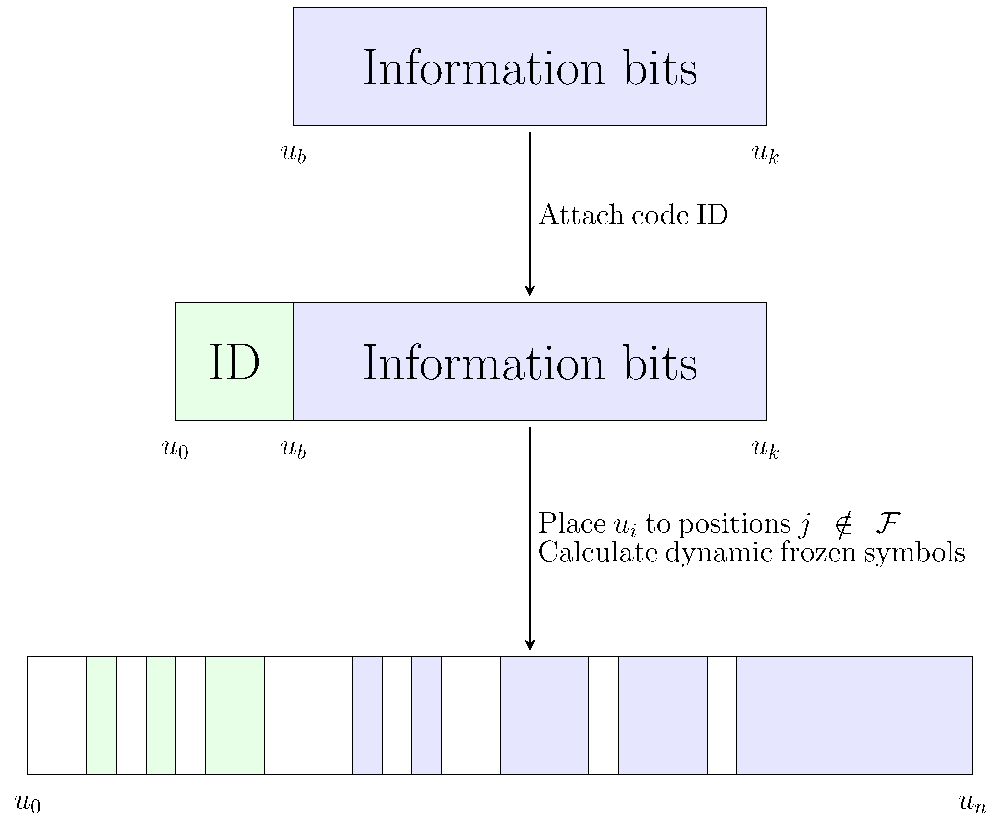
\includegraphics[width=0.7\linewidth]{pictures/BlindStructure.eps}
  \end{figure}
\end{frame}

%----------------------------------------------------------------------------------------
\begin{frame}{Сложность и задержка декодирования}
  \begin{table}
    \caption{Сложность декодирования $(1536, 768)$ кода, число операций}
    \begin{tabular}[c]{|l|ll|ll|}
      \hline
      & \multicolumn{2}{l|}{Сложения} & \multicolumn{2}{l|}{Сравнения}\\
      \hline
      $L$ & $A_m \otimes R_3$ & $A_{m'}$ & $A_m \otimes R_3$ & $A_{m'}$\\
      \hline
      1 & 3.5e+04 & 1.1e+04 & 2.1e+04 & 1.2e+04\\
      4 & 6.7e+04 & 4.2e+04 & 3.9e+04 & 5.0e+04\\
      8 & 9.8e+04 & 8.3e+04 & 5.5e+04 & 1.2e+05\\
      \hline
    \end{tabular}
  \end{table}

  Задержка декодирования $(1536, 768)$ кода предложенным списочным алгоритмом может быть уменьшена в $\approx 3$ раза по сравнению с классическим списочным алгоритмом декодирования полярных кодов
\end{frame}

%----------------------------------------------------------------------------------------
\begin{frame}{Summary}
  \begin{enumerate}
  \item PC based early termination scheme shows lower expected early termination phase than DCRC and Split-CRC schemes
  \item PC based scheme requires configuration of parameters depending on code used by the decoder
  \item DCRC scheme demonstrates the lowest FAR performance among all considered early termination schemes
  \item Additional parity checks can be used jointly with other early termination criterias to further lower expected early termination phase
  \end{enumerate}
\end{frame}

%----------------------------------------------------------------------------------------
\end{document} 

